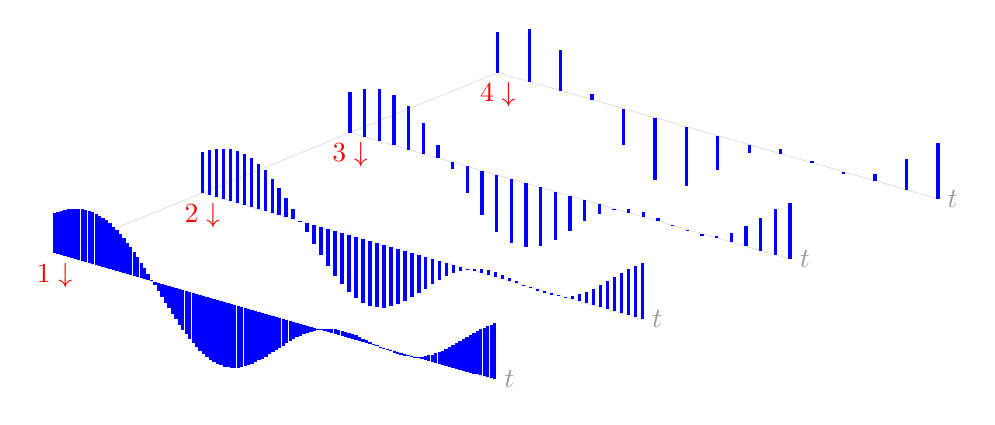
\begin{tikzpicture}[scale=1.8]
\begin{axis}[
    set layers=standard,
    domain=0:10,
    samples y=1,
    view={40}{20},
    hide axis,
    unit vector ratio*=1 2 1,
    xtick=\empty, ytick=\empty, ztick=\empty,
    clip=false
]

\draw [on layer=background, gray!20] (axis cs:0,2,0) -- (axis cs:0,8,0);
\pgfplotsinvokeforeach{1,2,3,4}{
    \draw (axis cs:0,#1*2,0) node[below, red]{$#1 \downarrow$} [on layer=background, gray!20]  -- (axis cs:10,#1*2,0) node[right, gray!80]{$t$};
    \addplot3 [on layer=main, blue!20, very thick, blue,ycomb,samples=256/2^#1]
      (x,#1*2,{1/2*sin(x*(75))+0.8*cos(x*(35)+20)});
}


\end{axis}
\end{tikzpicture}